
\section{Shape of a dusty radiative bow wave}
\label{sec:shape-dust-wave}

As an alternative to hydrodynamic or magnetohydrodynamic bow shocks,
it is possible that some observed emission arcs may be bow waves due
to the action of radiation pressure on dust grains.

\begin{figure}
  \centering
  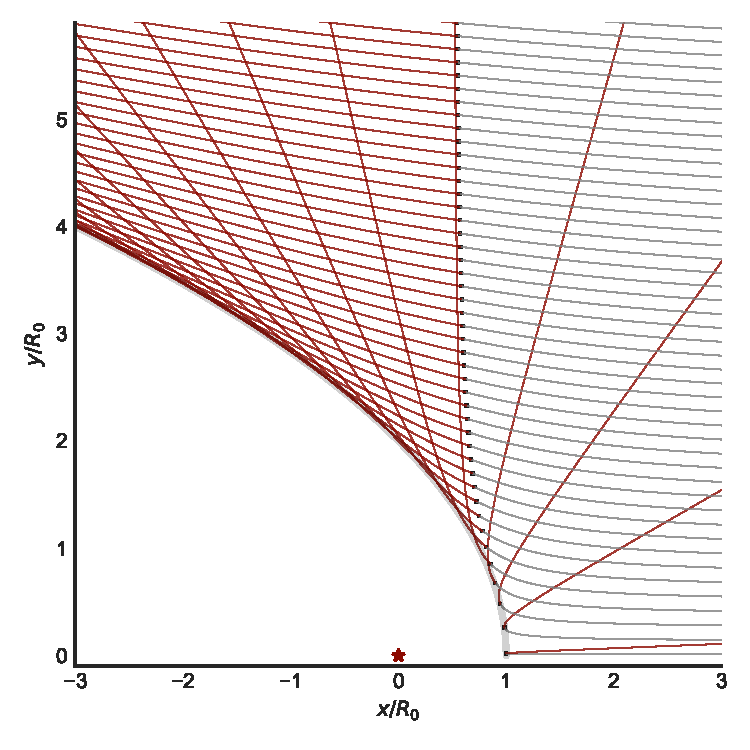
\includegraphics[width=\linewidth]{figs/dust-trajectories}
  \caption[Dust grain trajectories]{Dust grain trajectories under
    influence of a repulsive central \(r^{-2}\) radiative force.  Dust
    grains approach from the right at a uniform velocity and with a
    variety of impact parameters (initial \(y\)-coordinate). The
    central source is marked by a red star at the origin, and its
    radiative force deflects the trajectories into a hyperbolic shape,
    each of which reaches a minimum radius marked by a small black
    square.  The incoming hyperbolic trajectories are traced in gray
    and the outgoing trajectories are traced in red.  The locus of
    closest approach of the outgoing trajectories is parabolic in
    shape (traced by the thick, light gray line) and this constitutes
    the inner edge of the bow wave. }
  \label{fig:dust-trajectories}
\end{figure}



\newcommand\Qp{\ensuremath{Q_{\text{p}}}}
\newcommand{\grain}{\ensuremath{_{\text{g}}}}
\newcommand{\xsec}{\ensuremath{\sigma\grain}}
\newcommand\frad{\ensuremath{f_{\text{rad}}}}
\newcommand\thm{\ensuremath{\theta_{\text{m}}}}
A dust grain of geometrical cross-section \(\xsec\) situated a
distance \(R\) from a point source of radiation with luminosity \(L\)
will experience a repulsive, radially directed radiative force
\citep[e.g.,][]{Spitzer:1978a}
\begin{equation}
  \label{eq:dust-rad-force}
  \frad = \frac{\xsec \Qp L} {4 \pi R^2 c} e^{-\tau}
\end{equation}
where \Qp{} is the frequency-averaged\footnote{%
  Frequency averages of any quantity \(x\) should be understood as
  weighted by the attenuated source spectrum:
  \(\langle x \rangle_\nu = (L \, e^{-\tau})^{-1} \int_0^\infty x(\nu)\, L_\nu \, e^{-\tau_\nu} \, d\nu
  \).  } %
radiation pressure efficiency\footnote{%
  For absorption efficiency \(Q_{\text{abs}}\), scattering efficiency
  \(Q_{\text{scat}}\), and asymmetry parameter (mean scattering
  cosine) \(g\), we have
  \(\Qp = Q_{\text{abs}} + (1 - g) Q_{\text{scat}}\).  } %
of the grain, \(c\) is the speed of light, and \(\tau\) is the
frequency-averaged optical depth between the source and the grain.
For simplicity, we will consider only the optically thin case,
\(\tau \to 0\).

If \(\frad\) is the only force experienced by the grain, then it will
move on a \textit{ballistic} trajectory, determined by its initial
speed at large distance, \(u_\infty\), and its impact parameter, \(b\).
For \(b = 0\), the grain radially approaches the source with initial
radial velocity \(-u_\infty\), which is decelerated to zero at the distance
of closest approach, \(R_0\), given by energy conservation:
\begin{equation}
  \label{eq:dust-r0}
  R_0 = \frac{\xsec \Qp L} {2 \pi c m\grain u_\infty^2} \ ,
\end{equation}
where \(m\grain\) is the grain mass.  The grain then turns round and
recedes from the source along the same radius, reaching a velocity of
\(+u_\infty\) at large distance.  For \(b > 0\), the trajectory,
\(R(\theta)\), is readily found\footnote{%
  The problem is formally identical to that of Rutherford scattering,
  or (modulo a change of sign) planetary orbits.  The method of
  solution (via introduction of a centrifugal potential term and
  reduction to a 1-dimensional problem) can be found in any classical
  mechanics text \citep[e.g.,][\S~14]{Landau:1976a}. } in polar
coordinates as
\begin{equation}
  \label{eq:dust-r-theta}
  \frac{R\grain(\theta; b)} {R_0} = 
  \frac{ \tfrac12 \bigl( \varepsilon^2 - 1 \bigr)} {\varepsilon \cos(\theta - \thm) - 1}
\end{equation}
where \(\varepsilon^2 = 1 + 4 b^2 / R_0^2\) and
\(\thm = \cos^{-1} \varepsilon\) is the polar angle of closest approach along
the trajectory (see Fig.~\ref{fig:dust-trajectories}).  If the
incoming dust grains initially travel along parallel trajectories with
varying \(b\), but the same \(u_\infty\), then the deflection of the
trajectories by the radiative force will form a bow wave around the
radiation source, as shown in Figure~\ref{fig:dust-trajectories}.
However, the inner edge of the bow wave, \(R_{\text{in}}(\theta)\) is not
given by the closest approach along individual trajectories,
\(R\grain(\thm; b)\), but instead must found by minimizing
\(R\grain(\theta; b)\) over all \(b\) for each value of \(\theta\), which yields
\begin{equation}
  \label{eq:dust-r-in}
  \frac{R_{\text{in}}(\theta)} {R_0} = \frac{2}{1 + \cos\theta} \ .
\end{equation}
This is the polar form of the equation for the confocal parabola,
which we have already discussed in detail in \S~\ref{sec:conic} and
Appendix~\ref{app:parabola}.

\begin{figure*}
  \centering
  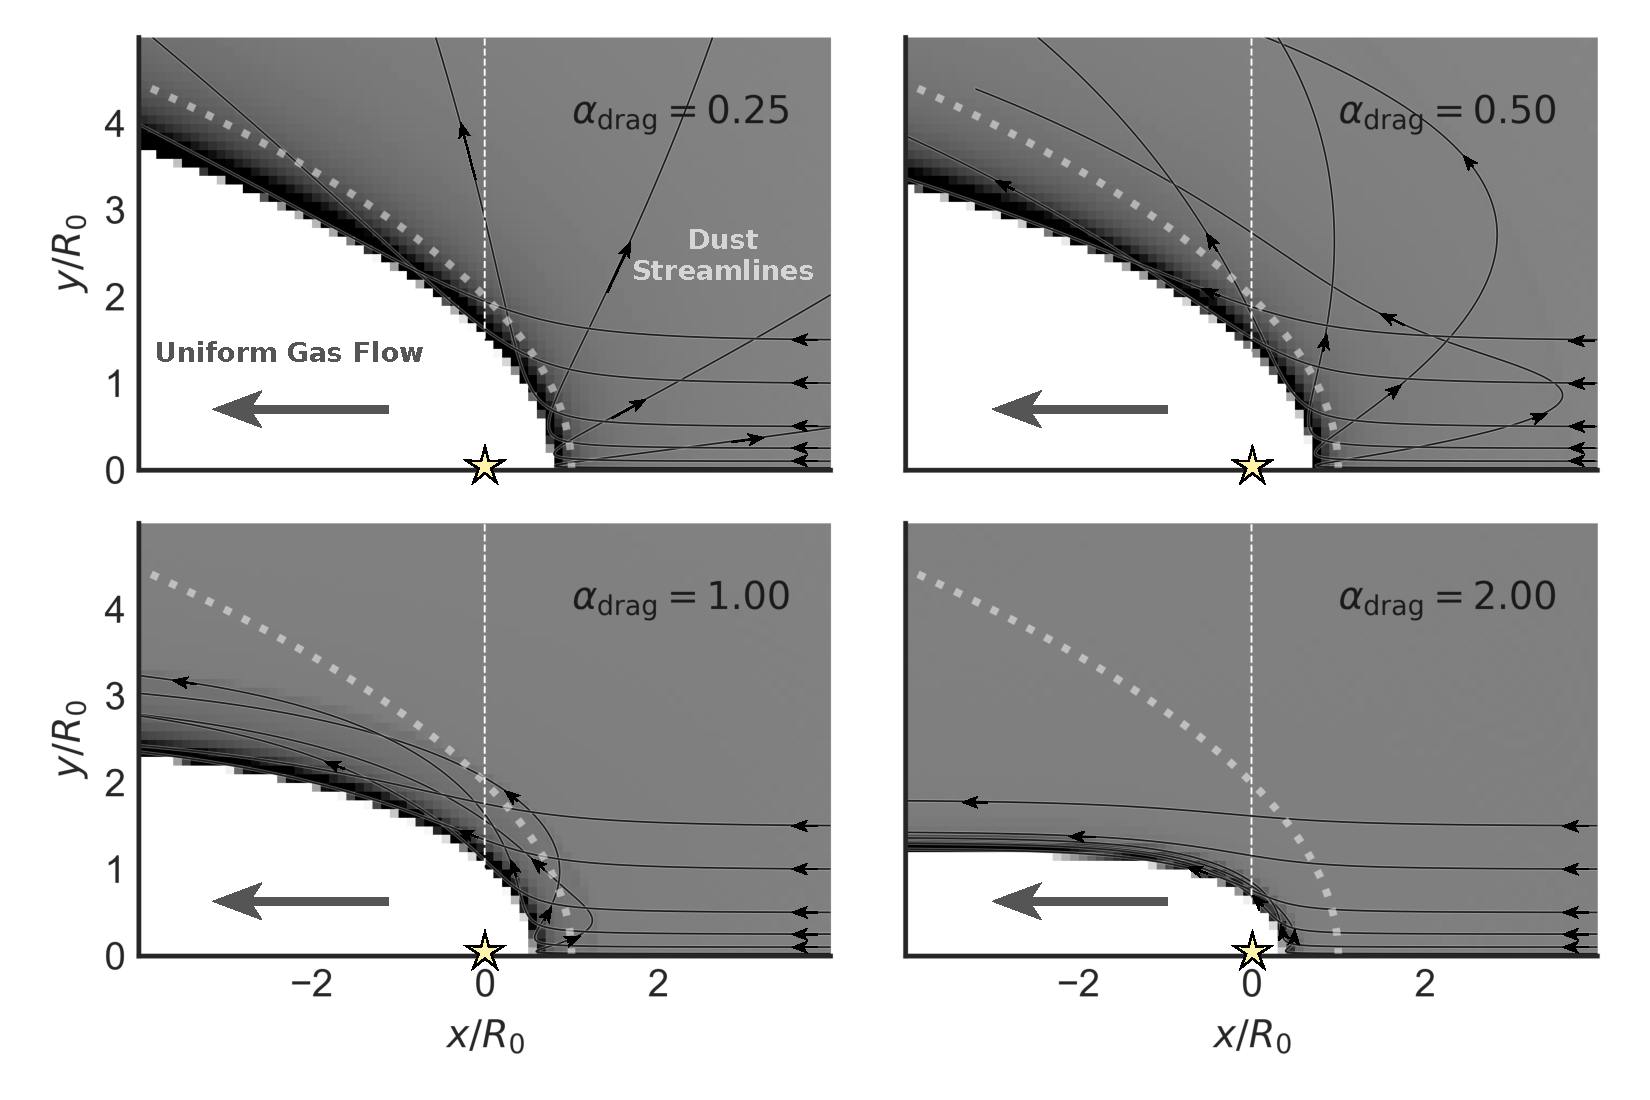
\includegraphics[width=\linewidth]{figs/dust-couple-stream-annotate}
  \caption{Dust grain trajectories under influence of gas drag in
    addition a repulsive central radiative force.  The dust
    streamlines are shown in blue and the dust density as a linear
    color scale, with maximum (white-yellow) of twice the ambient dust
    density.  Results are shown for four values of the drag parameter
    (see text): \(\alpha_\text{drag} = 0.25\), \(0.5\), \(1.0\), and
    \(2.0\). The shape of the bow wave for the drag-free case
    (Fig.~\ref{fig:dust-trajectories}) is shown by the thick dotted
    line.}
  \label{fig:dust-wave-coupling}
\end{figure*}


\begin{figure}
  \centering
  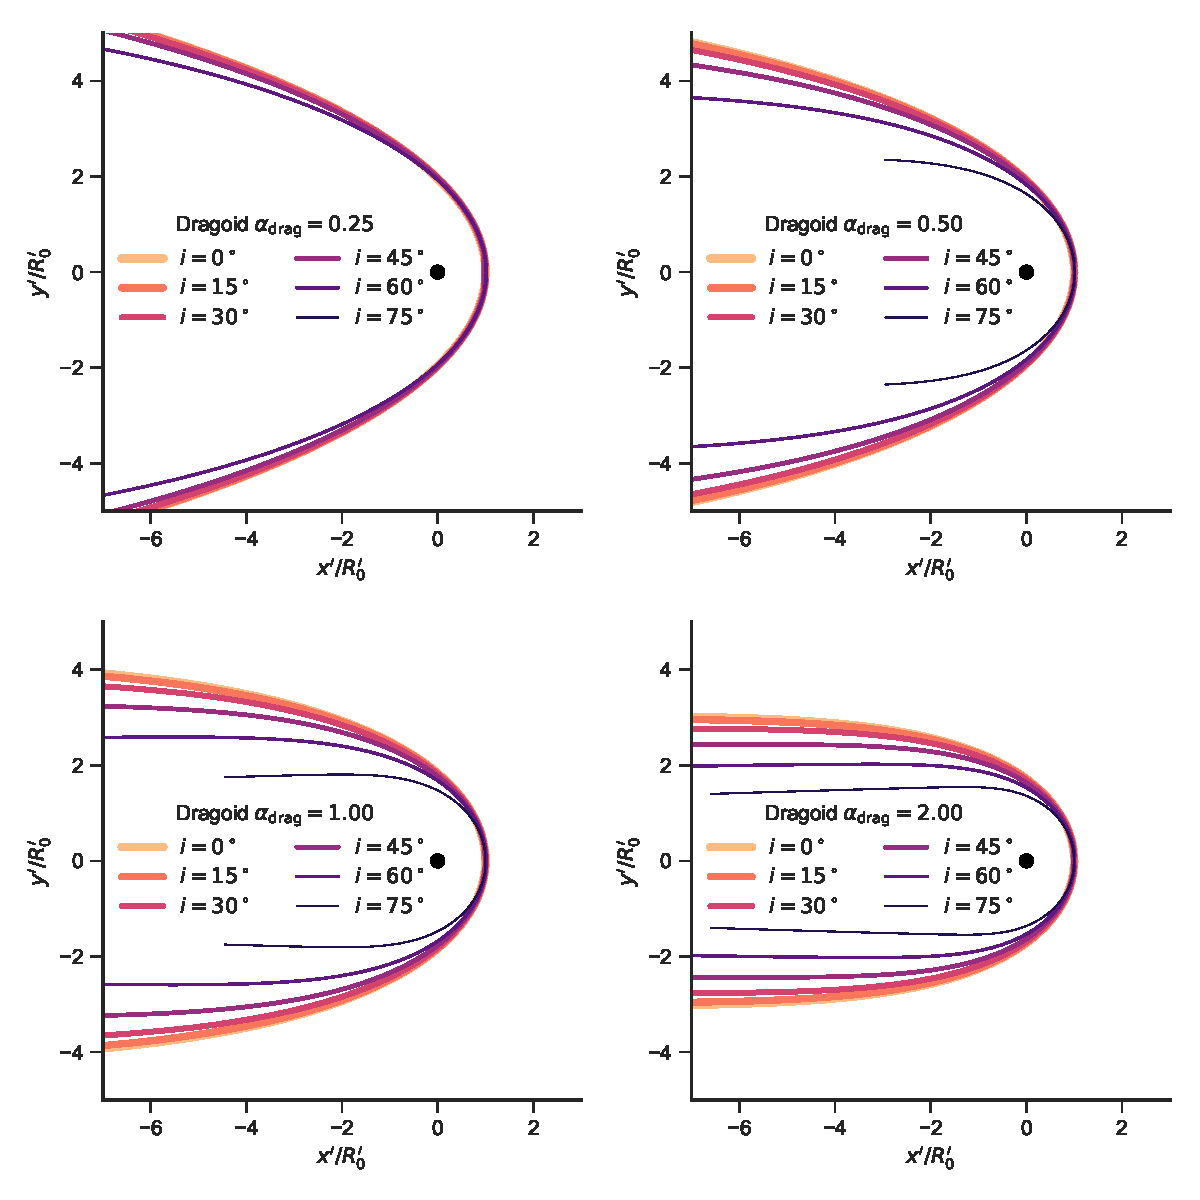
\includegraphics[width=\linewidth]{figs/test_xyprime_dragoid}
  \caption{Plane-of-sky shapes for dragoids.}
  \label{fig:dragoid-xy-prime}
\end{figure}


\begin{figure}
  \centering
  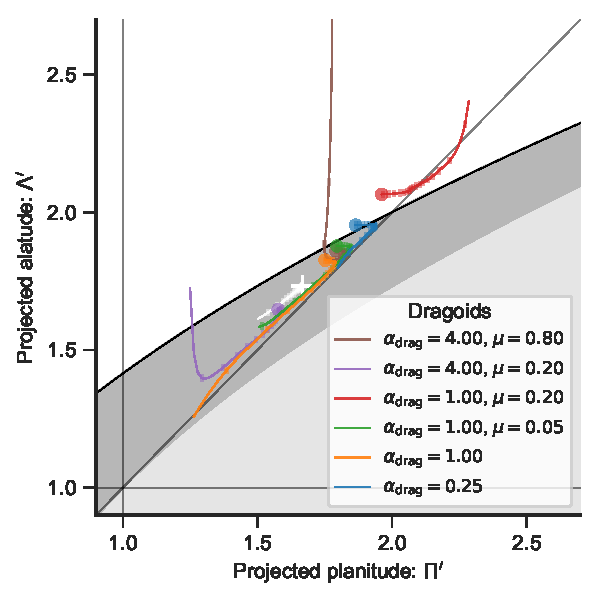
\includegraphics[width=\linewidth]{figs/dragoid-R90-vs-Rc}
  \caption{Diagnostic diagram for dragoids}
  \label{fig:dragoid-Rc-R90}
\end{figure}

%%% Local Variables:
%%% mode: latex
%%% TeX-master: "quadrics-bowshock"
%%% End:
